% Options for packages loaded elsewhere
\PassOptionsToPackage{unicode}{hyperref}
\PassOptionsToPackage{hyphens}{url}
%
\documentclass[
]{article}
\usepackage{amsmath,amssymb}
\usepackage{lmodern}
\usepackage{iftex}
\ifPDFTeX
  \usepackage[T1]{fontenc}
  \usepackage[utf8]{inputenc}
  \usepackage{textcomp} % provide euro and other symbols
\else % if luatex or xetex
  \usepackage{unicode-math}
  \defaultfontfeatures{Scale=MatchLowercase}
  \defaultfontfeatures[\rmfamily]{Ligatures=TeX,Scale=1}
\fi
% Use upquote if available, for straight quotes in verbatim environments
\IfFileExists{upquote.sty}{\usepackage{upquote}}{}
\IfFileExists{microtype.sty}{% use microtype if available
  \usepackage[]{microtype}
  \UseMicrotypeSet[protrusion]{basicmath} % disable protrusion for tt fonts
}{}
\makeatletter
\@ifundefined{KOMAClassName}{% if non-KOMA class
  \IfFileExists{parskip.sty}{%
    \usepackage{parskip}
  }{% else
    \setlength{\parindent}{0pt}
    \setlength{\parskip}{6pt plus 2pt minus 1pt}}
}{% if KOMA class
  \KOMAoptions{parskip=half}}
\makeatother
\usepackage{xcolor}
\usepackage[margin=1in]{geometry}
\usepackage{color}
\usepackage{fancyvrb}
\newcommand{\VerbBar}{|}
\newcommand{\VERB}{\Verb[commandchars=\\\{\}]}
\DefineVerbatimEnvironment{Highlighting}{Verbatim}{commandchars=\\\{\}}
% Add ',fontsize=\small' for more characters per line
\usepackage{framed}
\definecolor{shadecolor}{RGB}{248,248,248}
\newenvironment{Shaded}{\begin{snugshade}}{\end{snugshade}}
\newcommand{\AlertTok}[1]{\textcolor[rgb]{0.94,0.16,0.16}{#1}}
\newcommand{\AnnotationTok}[1]{\textcolor[rgb]{0.56,0.35,0.01}{\textbf{\textit{#1}}}}
\newcommand{\AttributeTok}[1]{\textcolor[rgb]{0.77,0.63,0.00}{#1}}
\newcommand{\BaseNTok}[1]{\textcolor[rgb]{0.00,0.00,0.81}{#1}}
\newcommand{\BuiltInTok}[1]{#1}
\newcommand{\CharTok}[1]{\textcolor[rgb]{0.31,0.60,0.02}{#1}}
\newcommand{\CommentTok}[1]{\textcolor[rgb]{0.56,0.35,0.01}{\textit{#1}}}
\newcommand{\CommentVarTok}[1]{\textcolor[rgb]{0.56,0.35,0.01}{\textbf{\textit{#1}}}}
\newcommand{\ConstantTok}[1]{\textcolor[rgb]{0.00,0.00,0.00}{#1}}
\newcommand{\ControlFlowTok}[1]{\textcolor[rgb]{0.13,0.29,0.53}{\textbf{#1}}}
\newcommand{\DataTypeTok}[1]{\textcolor[rgb]{0.13,0.29,0.53}{#1}}
\newcommand{\DecValTok}[1]{\textcolor[rgb]{0.00,0.00,0.81}{#1}}
\newcommand{\DocumentationTok}[1]{\textcolor[rgb]{0.56,0.35,0.01}{\textbf{\textit{#1}}}}
\newcommand{\ErrorTok}[1]{\textcolor[rgb]{0.64,0.00,0.00}{\textbf{#1}}}
\newcommand{\ExtensionTok}[1]{#1}
\newcommand{\FloatTok}[1]{\textcolor[rgb]{0.00,0.00,0.81}{#1}}
\newcommand{\FunctionTok}[1]{\textcolor[rgb]{0.00,0.00,0.00}{#1}}
\newcommand{\ImportTok}[1]{#1}
\newcommand{\InformationTok}[1]{\textcolor[rgb]{0.56,0.35,0.01}{\textbf{\textit{#1}}}}
\newcommand{\KeywordTok}[1]{\textcolor[rgb]{0.13,0.29,0.53}{\textbf{#1}}}
\newcommand{\NormalTok}[1]{#1}
\newcommand{\OperatorTok}[1]{\textcolor[rgb]{0.81,0.36,0.00}{\textbf{#1}}}
\newcommand{\OtherTok}[1]{\textcolor[rgb]{0.56,0.35,0.01}{#1}}
\newcommand{\PreprocessorTok}[1]{\textcolor[rgb]{0.56,0.35,0.01}{\textit{#1}}}
\newcommand{\RegionMarkerTok}[1]{#1}
\newcommand{\SpecialCharTok}[1]{\textcolor[rgb]{0.00,0.00,0.00}{#1}}
\newcommand{\SpecialStringTok}[1]{\textcolor[rgb]{0.31,0.60,0.02}{#1}}
\newcommand{\StringTok}[1]{\textcolor[rgb]{0.31,0.60,0.02}{#1}}
\newcommand{\VariableTok}[1]{\textcolor[rgb]{0.00,0.00,0.00}{#1}}
\newcommand{\VerbatimStringTok}[1]{\textcolor[rgb]{0.31,0.60,0.02}{#1}}
\newcommand{\WarningTok}[1]{\textcolor[rgb]{0.56,0.35,0.01}{\textbf{\textit{#1}}}}
\usepackage{longtable,booktabs,array}
\usepackage{calc} % for calculating minipage widths
% Correct order of tables after \paragraph or \subparagraph
\usepackage{etoolbox}
\makeatletter
\patchcmd\longtable{\par}{\if@noskipsec\mbox{}\fi\par}{}{}
\makeatother
% Allow footnotes in longtable head/foot
\IfFileExists{footnotehyper.sty}{\usepackage{footnotehyper}}{\usepackage{footnote}}
\makesavenoteenv{longtable}
\usepackage{graphicx}
\makeatletter
\def\maxwidth{\ifdim\Gin@nat@width>\linewidth\linewidth\else\Gin@nat@width\fi}
\def\maxheight{\ifdim\Gin@nat@height>\textheight\textheight\else\Gin@nat@height\fi}
\makeatother
% Scale images if necessary, so that they will not overflow the page
% margins by default, and it is still possible to overwrite the defaults
% using explicit options in \includegraphics[width, height, ...]{}
\setkeys{Gin}{width=\maxwidth,height=\maxheight,keepaspectratio}
% Set default figure placement to htbp
\makeatletter
\def\fps@figure{htbp}
\makeatother
\setlength{\emergencystretch}{3em} % prevent overfull lines
\providecommand{\tightlist}{%
  \setlength{\itemsep}{0pt}\setlength{\parskip}{0pt}}
\setcounter{secnumdepth}{-\maxdimen} % remove section numbering
\ifLuaTeX
  \usepackage{selnolig}  % disable illegal ligatures
\fi
\IfFileExists{bookmark.sty}{\usepackage{bookmark}}{\usepackage{hyperref}}
\IfFileExists{xurl.sty}{\usepackage{xurl}}{} % add URL line breaks if available
\urlstyle{same} % disable monospaced font for URLs
\hypersetup{
  pdftitle={PSTAT 174/274: Homework \# 1},
  pdfauthor={Dylan Berneman},
  hidelinks,
  pdfcreator={LaTeX via pandoc}}

\title{PSTAT 174/274: Homework \# 1}
\author{Dylan Berneman}
\date{2023-04-14}

\begin{document}
\maketitle

This homework is based on Lectures 1--2. Please study material of week 1
before starting working on this problems. Good Luck!

\hypertarget{question-1}{%
\paragraph{Question 1}\label{question-1}}

\emph{Understanding deterministic and stochastic trends.} You are given
the following statements about time series:

\setlength{\leftskip}{2cm}

\begin{itemize}
\item
  \begin{enumerate}
  \def\labelenumi{\Roman{enumi}.}
  \tightlist
  \item
    Stochastic trends are characterized by explainable changes in
    direction.\\
  \end{enumerate}
\item
  \begin{enumerate}
  \def\labelenumi{\Roman{enumi}.}
  \setcounter{enumi}{1}
  \tightlist
  \item
    Deterministic trends are better suited to extrapolation than
    stochastic trends.\\
  \end{enumerate}
\item
  \begin{enumerate}
  \def\labelenumi{\Roman{enumi}.}
  \setcounter{enumi}{2}
  \tightlist
  \item
    Short term extrapolation of deterministic trends can be justified by
    claiming that underlying trends will usually change slowly in
    comparison with the forecast lead time.
  \end{enumerate}
\end{itemize}

\setlength{\leftskip}{0cm}

Determine which statements are true. Explain.\\

\setlength{\leftskip}{2cm}

~~~~~~~~A. I only\\
\hspace*{0.333em}\hspace*{0.333em}\hspace*{0.333em}\hspace*{0.333em}\hspace*{0.333em}\hspace*{0.333em}\hspace*{0.333em}\hspace*{0.333em}B.
II only\\
\hspace*{0.333em}\hspace*{0.333em}\hspace*{0.333em}\hspace*{0.333em}\hspace*{0.333em}\hspace*{0.333em}\hspace*{0.333em}\hspace*{0.333em}C.
III only\\
\hspace*{0.333em}\hspace*{0.333em}\hspace*{0.333em}\hspace*{0.333em}\hspace*{0.333em}\hspace*{0.333em}\hspace*{0.333em}\hspace*{0.333em}D.
I, II, and III\\
\hspace*{0.333em}\hspace*{0.333em}\hspace*{0.333em}\hspace*{0.333em}\hspace*{0.333em}\hspace*{0.333em}\hspace*{0.333em}\hspace*{0.333em}E.
The answer is not given by (A), (B), (C), or (D).

\setlength{\leftskip}{0cm}\\

\setlength{\leftskip}{2cm}

\begin{enumerate}
\def\labelenumi{\Roman{enumi}.}
\item
  False. Stochastic trends are characterized by unexplainable changes in
  direction. They arise from the random movement of the variable over
  time.
\item
  True. Deterministic trends are a result of the constant effect of a
  few causal forces an are generally stable over time.
\item
  True. Deterministic trends can provide accurate forecasts for several
  periods ahead, as forecasting generally assumes that trends will
  continue and change relatively slowly.
\end{enumerate}

\hypertarget{question-2}{%
\paragraph{Question 2}\label{question-2}}

\emph{Random walk and stationarity. In this question we introduce WN and
random walk with non-zero mean. A White Noise with non-zero mean}\\
Z\textsubscript{t} ∼ WN(μ\textsubscript{Z},
σ\textsuperscript{2}\textsubscript{Z}), \emph{is a collection of
uncorrelated random variables with the same mean and variance:}
E(Z\textsubscript{t}) = μ\textsubscript{Z}, Var(Z\textsubscript{t}) =
σ\textsubscript{Z}\textsuperscript{2}, and Cov(Z\textsubscript{t},
Z\textsubscript{s}) = 0 for t \(\ne\) s. \emph{When} Z\textsubscript{t}
\emph{is referred to as a `White Noise', without specifying its mean, by
default, assume} μ\textsubscript{Z} = 0. \emph{A random walk with
non-zero mean is expressed as} X\textsubscript{1} =Z\textsubscript{1},
X\textsubscript{t} = X\textsubscript{t−1} + Z\textsubscript{t} =
Z\textsubscript{1}+\ldots+Z\textsubscript{t}, t=2,3,\ldots, \emph{where}
Z\textsubscript{t} ∼WN(μ\textsubscript{Z},
σ\textsubscript{Z}\textsuperscript{2}).\\
Determine which statements are true with respect to a random walk model;
show calculations and provide complete explanations.~
\setlength{\leftskip}{2cm}

\begin{itemize}
\item
  \begin{enumerate}
  \def\labelenumi{\Roman{enumi}.}
  \tightlist
  \item
    If μ\textsubscript{Z} \(\neq\) 0, then the random walk is
    nonstationary in the mean.\\
    \emph{(Hint: Nonstationary in the mean means that the mean changes
    with time.)}
  \end{enumerate}
\item
  \begin{enumerate}
  \def\labelenumi{\Roman{enumi}.}
  \setcounter{enumi}{1}
  \tightlist
  \item
    If σ\textsubscript{Z}\textsuperscript{2} = 0, then the random walk
    is nonstationary in the variance.\\
    \emph{(Hint: Nonstationary in the variance means that the variance
    changes with time.)}
  \end{enumerate}
\item
  \begin{enumerate}
  \def\labelenumi{\Roman{enumi}.}
  \setcounter{enumi}{2}
  \tightlist
  \item
    If σ\textsubscript{Z}\textsuperscript{2} \textgreater{} 0, then the
    random walk is nonstationary in the variance.\\
  \end{enumerate}
\end{itemize}

\setlength{\leftskip}{0cm}

\setlength{\leftskip}{2cm}

\begin{verbatim}
I. True. 
\end{verbatim}

~~~~~~~~For all t where t \(\ge\) 1, E{[}X\textsubscript{t}{]} =
E{[}X\textsubscript{t-1}{]} + Z\textsubscript{t}

\[ 
\begin{align*}
  E[Z_{t}] & = E[Z_{1}] = E[Z_{2}] = E[Z_{t-1}] = E[Z_{t}] =  \mu_{Z} \\
  E[X_{t}] & = E[Z_{1}] + E[Z_{2}] + ... E[Z_{t-1}] + E[Z_{t}] \\
  & = tE[Z_{t}] \\
  & = t\mu_{Z} \\
\end{align*} 
\] \[
\begin{aligned}
& E[X_{1}] = E[Z_{1}] = \mu_{Z}\\
& E[X_{2}] = E[X_{1}] + E[Z_{2}] = 2\mu_{Z}\\
& E[X_{t-1}] = E[X_{t-2}] + E[Z_{t-1}] = (t-1)\mu_{Z}\\
& E[X_{t}] = E[X_{t-1}] + E[Z_{t}] = t\mu_{Z}\\ \\
& Therefore,\ E[X_{1}] \neq E[X_{2}] \neq E[X_{t-1}] \neq E[X_{t}]
\end{aligned} 
\]

Since \(\mu_{Z} > 0\ \ or \ \ \mu_{Z} < 0,\ X_{t}\) either increases or
decreases by increments of \(\mu_{Z}\)\\
Thus the random walk is nonstationary in the mean.

\begin{verbatim}
II. False
\end{verbatim}

\[
\begin{aligned}
& \text{It is given that}\ σ_{Z}^2=0\  \ \ \ \& \ \ \ Cov(Z_{t}, Z_{s}) =0,\ for\ t \ne s 
\end{aligned}
\] \[ 
\begin{aligned}
For\ all\ &t\ \ge 1,\ Var[X_{t}] = Var[X_{t-1} + Z_{t}]\\
Var[Z_{t}] & = Var[Z_{1}] = Var[Z_{2}] = Var[Z_{t-1}] = Var[Z_{t}] =  \sigma^2_{Z} =0 \\ \\
Var[X_{1}]& = Var[Z_{1}] = \sigma^2_{Z} = 0\\
Var[X_{2}]& = Var[X_{1} + Z_{2}] \\
&= Var[X_{1}] + Var[Z_{2}] + 2Cov[X_{1}, Z_{2}]\\
&= Var[X_{1}] + Var[Z_{2}] + 2Cov[Z_{1}, Z_{2}]\\
&= 0 + 0 + 2(0)\\
&=0\\
Var[X_{t-1}]& = Var[X_{t-2} + Z_{t-1}] \\
&= Var[X_{t-2}] + Var[Z_{t-1}] + 2Cov[X_{t-2}, Z_{t-1}]\\
&= Var[X_{t-2}] + Var[Z_{t-1}] + 2Cov[Z_{t-2}, Z_{t-1}]\\
&= 0 + 0 + 2(0)\\
&=0\\
Var[X_{t}]& = Var[X_{t-1} + Z_{t}] \\
&= Var[X_{t-1}] + Var[Z_{t}] + 2Cov[X_{t-1}, Z_{t}]\\
&= Var[X_{t-1}] + Var[Z_{t}] + 2Cov[Z_{t-1}, Z_{t}]\\
&= 0 + 0 + 2(0)\\
&=0\\
& Therefore,\ Var[X_{1}] = Var[X_{2}] = Var[X_{t-1}] = Var[X_{t}]\\
& \text{Thus, the random walk is stationary in the variance}\\
& \text{because the variance remains constant as t changes.}
\end{aligned} 
\]\\

\begin{verbatim}
III. True
\end{verbatim}

\[ \text{It is given that}\ σ_{Z}^2>0\  \ \ \ \& \ \ \ Cov(Z_{t}, Z_{s}) =0,\ for\ t \ne s\]
\[ 
\begin{aligned}
For\ all\ &t\ \ge 1,\ Var[X_{t}] = Var[X_{t-1} + Z_{t}]\\
Var[Z_{t}] & = Var[Z_{1}] = Var[Z_{2}] = Var[Z_{t-1}] = Var[Z_{t}] =  \sigma^2_{Z} \\ \\
Var[X_{1}]& = Var[Z_{1}] = \sigma^2_{Z}\\
Var[X_{2}]& = Var[X_{1} + Z_{2}] \\
&= Var[X_{1}] + Var[Z_{2}] + 2Cov[X_{1}, Z_{2}]\\
&= Var[Z_{1}] + Var[Z_{2}] + 2Cov[Z_{1}, Z_{2}]\\
&= \sigma^2_{Z} + \sigma^2_{Z} + 2(0)\\
&= 2\sigma^2_{Z} \\ \\
& \text{This implies that}\ Var[X_{2}] = 2Var[X_{1}] = 2Var[Z_{1}]\\ \\
Var[X_{3}]& = Var[X_{2} + Z_{3}] \\
&= Var[X_{2}] + Var[Z_{3}] + 2Cov[X_{2}, Z_{3}]\\
&= 2Var[Z_{2}] + Var[Z_{3}] + 2Cov[2*Z_{2}, Z_{3}]\\
&= 2\sigma^2_{Z} + \sigma^2_{Z} + 2(2)(0)\\
&= 3\sigma^2_{Z} \\ \\
Var[X_{t}]& = Var[X_{t-1} + Z_{t}] \\
&= Var[X_{t-1}] + Var[Z_{t}] + 2Cov[X_{t-1}, Z_{t}]\\
&= 2Var[Z_{t-1}] + Var[Z_{t}] + 2Cov[(t-1)*Z_{t-1}, Z_{t}]\\
&= (t-1)\sigma^2_{Z} + \sigma^2_{Z} + 2(t-1)(0)\\
&= t\sigma^2_{Z} \\ \\
& \text{Therefore},\ Var[X_{1}] \ne Var[X_{2}] \ne Var[X_{3}] \ne Var[X_{t}]\\
& \text{Thus, the random walk is nonstationary in the variance}\\
& \text{because the variance increases by increments of}\ Var[Z_{t}]\ \text{as t changes}.
\end{aligned} 
\]

\setlength{\leftskip}{0cm}\\

\hypertarget{question-3}{%
\paragraph{Question 3}\label{question-3}}

\emph{Calculation of sample acf.} You are given the following stock
prices of company CAS:

\begin{longtable}[]{@{}cc@{}}
\toprule()
Day & Stock Price \\
\midrule()
\endhead
1 & 538 \\
2 & 548 \\
3 & 528 \\
4 & 608 \\
5 & 598 \\
6 & 589 \\
7 & 548 \\
8 & 514 \\
9 & 501 \\
10 & 498 \\
\bottomrule()
\end{longtable}

Calculate the sample autocorrelation at lag 3.\\
\emph{Hints:}\\
\setlength{\leftskip}{2cm}

\emph{(i) We are given a sample of size n = 10 to estimate
autocorrelation at lag 3:} ρ(3) = Cor(X\textsubscript{1},
X\textsubscript{4}) = \(\frac{γ(3)}{γ(0)}\)\\
\emph{-- for definition of autocorrelation at lag 3 see Week 1 slide 52
or (2.1.3) on p.6 of Lecture Notes.}\\
\emph{(ii) General formulas for calculating sample mean and covariance
are given on slide 38 of week 1 and in §1.2 on p.4 of Lecture notes for
week 1.} \emph{To estimate} ρ(3) = Cor(X\textsubscript{1},
X\textsubscript{4}) \emph{we have:}\\
\[\bar{x}=\frac{1}{n} \sum_{t=1}^n x_t, \quad \hat{\rho}_3=\frac{\hat{\gamma}(3)}{\hat{\gamma}(0)}=\frac{\sum_{t=1}^{n-3}\left(x_t-\bar{x}\right)\left(x_{t+3}-\bar{x}\right)}{\sum_{t=1}^n\left(x_t-\bar{x}\right)^2}\]

\begin{Shaded}
\begin{Highlighting}[]
\NormalTok{data }\OtherTok{=} \FunctionTok{data.frame}\NormalTok{(}\FunctionTok{matrix}\NormalTok{(}\AttributeTok{ncol=}\DecValTok{5}\NormalTok{, }\AttributeTok{nrow=}\DecValTok{10}\NormalTok{))}
\FunctionTok{colnames}\NormalTok{(data)}\OtherTok{\textless{}{-}}\FunctionTok{c}\NormalTok{(}\StringTok{"Day"}\NormalTok{, }\StringTok{"SP ($x\_\{t\}$)"}\NormalTok{, }\StringTok{"$(x\_\{t\}{-} }\SpecialCharTok{\textbackslash{}\textbackslash{}}\StringTok{bar\{x\})$"}\NormalTok{, }\StringTok{"$(x\_\{t\}{-} }\SpecialCharTok{\textbackslash{}\textbackslash{}}\StringTok{bar\{x\})\^{}2$"}\NormalTok{, }\StringTok{"$(x\_\{t\}{-} }\SpecialCharTok{\textbackslash{}\textbackslash{}}\StringTok{bar\{x\})(x\_\{t+3\}\textbackslash{} \textbackslash{} {-} \textbackslash{} }\SpecialCharTok{\textbackslash{}\textbackslash{}}\StringTok{bar\{x\})$"}\NormalTok{)}

\NormalTok{data}\SpecialCharTok{$}\NormalTok{Day }\OtherTok{\textless{}{-}} \FunctionTok{c}\NormalTok{(}\FunctionTok{seq}\NormalTok{(}\DecValTok{1}\NormalTok{,}\DecValTok{10}\NormalTok{))}
\NormalTok{data[,}\DecValTok{2}\NormalTok{] }\OtherTok{\textless{}{-}} \FunctionTok{c}\NormalTok{(}\DecValTok{538}\NormalTok{, }\DecValTok{548}\NormalTok{, }\DecValTok{528}\NormalTok{, }\DecValTok{608}\NormalTok{, }\DecValTok{598}\NormalTok{, }\DecValTok{589}\NormalTok{, }\DecValTok{548}\NormalTok{, }\DecValTok{514}\NormalTok{, }\DecValTok{501}\NormalTok{, }\DecValTok{498}\NormalTok{)}

\NormalTok{mean }\OtherTok{=} \FunctionTok{mean}\NormalTok{(data[,}\DecValTok{2}\NormalTok{])}
\ControlFlowTok{for}\NormalTok{(i }\ControlFlowTok{in} \DecValTok{1}\SpecialCharTok{:}\DecValTok{10}\NormalTok{)\{}
\NormalTok{  data[i,}\DecValTok{3}\NormalTok{] }\OtherTok{=}\NormalTok{ data[i,}\DecValTok{2}\NormalTok{] }\SpecialCharTok{{-}}\NormalTok{ mean\}}

\ControlFlowTok{for}\NormalTok{(i }\ControlFlowTok{in} \DecValTok{1}\SpecialCharTok{:}\DecValTok{10}\NormalTok{)\{}
\NormalTok{  data[i,}\DecValTok{4}\NormalTok{] }\OtherTok{=}\NormalTok{ (data[i,}\DecValTok{2}\NormalTok{] }\SpecialCharTok{{-}}\NormalTok{ mean)}\SpecialCharTok{\^{}}\DecValTok{2}\NormalTok{\}}

\NormalTok{data[,}\DecValTok{5}\NormalTok{] }\OtherTok{\textless{}{-}} \ConstantTok{NA}
\ControlFlowTok{for}\NormalTok{(i }\ControlFlowTok{in} \DecValTok{1}\SpecialCharTok{:}\DecValTok{7}\NormalTok{)\{}
\NormalTok{  data[i,}\DecValTok{5}\NormalTok{] }\OtherTok{=}\NormalTok{ data[i, }\DecValTok{3}\NormalTok{] }\SpecialCharTok{*}\NormalTok{ data[i}\SpecialCharTok{+}\DecValTok{3}\NormalTok{, }\DecValTok{3}\NormalTok{]\}}

\NormalTok{data[}\DecValTok{11}\NormalTok{,}\DecValTok{1}\NormalTok{] }\OtherTok{\textless{}{-}} \StringTok{"total"}
\NormalTok{data[}\DecValTok{11}\NormalTok{,}\DecValTok{2}\NormalTok{] }\OtherTok{\textless{}{-}} \FunctionTok{sum}\NormalTok{(}\FunctionTok{as.integer}\NormalTok{(data[}\DecValTok{1}\SpecialCharTok{:}\DecValTok{10}\NormalTok{, }\DecValTok{2}\NormalTok{]))}
\NormalTok{data[}\DecValTok{11}\NormalTok{,}\DecValTok{3}\NormalTok{] }\OtherTok{\textless{}{-}} \FunctionTok{sum}\NormalTok{(}\FunctionTok{as.integer}\NormalTok{(data[}\DecValTok{1}\SpecialCharTok{:}\DecValTok{10}\NormalTok{, }\DecValTok{3}\NormalTok{]))}
\NormalTok{data[}\DecValTok{11}\NormalTok{,}\DecValTok{4}\NormalTok{] }\OtherTok{\textless{}{-}} \FunctionTok{sum}\NormalTok{(}\FunctionTok{as.integer}\NormalTok{(data[}\DecValTok{1}\SpecialCharTok{:}\DecValTok{10}\NormalTok{, }\DecValTok{4}\NormalTok{]))}
\NormalTok{data[}\DecValTok{11}\NormalTok{,}\DecValTok{5}\NormalTok{] }\OtherTok{\textless{}{-}} \FunctionTok{sum}\NormalTok{(}\FunctionTok{as.integer}\NormalTok{(data[}\DecValTok{1}\SpecialCharTok{:}\DecValTok{7}\NormalTok{, }\DecValTok{5}\NormalTok{]))}
\NormalTok{knitr}\SpecialCharTok{::}\FunctionTok{kable}\NormalTok{(data)}
\end{Highlighting}
\end{Shaded}

\begin{longtable}[]{@{}
  >{\raggedright\arraybackslash}p{(\columnwidth - 8\tabcolsep) * \real{0.0606}}
  >{\raggedleft\arraybackslash}p{(\columnwidth - 8\tabcolsep) * \real{0.1313}}
  >{\raggedleft\arraybackslash}p{(\columnwidth - 8\tabcolsep) * \real{0.1919}}
  >{\raggedleft\arraybackslash}p{(\columnwidth - 8\tabcolsep) * \real{0.2121}}
  >{\raggedleft\arraybackslash}p{(\columnwidth - 8\tabcolsep) * \real{0.4040}}@{}}
\toprule()
\begin{minipage}[b]{\linewidth}\raggedright
Day
\end{minipage} & \begin{minipage}[b]{\linewidth}\raggedleft
SP (\(x_{t}\))
\end{minipage} & \begin{minipage}[b]{\linewidth}\raggedleft
\((x_{t}- \bar{x})\)
\end{minipage} & \begin{minipage}[b]{\linewidth}\raggedleft
\((x_{t}- \bar{x})^2\)
\end{minipage} & \begin{minipage}[b]{\linewidth}\raggedleft
\((x_{t}- \bar{x})(x_{t+3} - \bar{x})\)
\end{minipage} \\
\midrule()
\endhead
1 & 538 & -9 & 81 & -549 \\
2 & 548 & 1 & 1 & 51 \\
3 & 528 & -19 & 361 & -798 \\
4 & 608 & 61 & 3721 & 61 \\
5 & 598 & 51 & 2601 & -1683 \\
6 & 589 & 42 & 1764 & -1932 \\
7 & 548 & 1 & 1 & -49 \\
8 & 514 & -33 & 1089 & NA \\
9 & 501 & -46 & 2116 & NA \\
10 & 498 & -49 & 2401 & NA \\
total & 5470 & 0 & 14136 & -4899 \\
\bottomrule()
\end{longtable}

\begin{Shaded}
\begin{Highlighting}[]
\CommentTok{\# Autocorrelation}
\NormalTok{data[}\DecValTok{11}\NormalTok{,}\DecValTok{5}\NormalTok{] }\SpecialCharTok{/}\NormalTok{ data[}\DecValTok{11}\NormalTok{,}\DecValTok{4}\NormalTok{]}
\end{Highlighting}
\end{Shaded}

\begin{verbatim}
## [1] -0.346562
\end{verbatim}

\hfill\break
\hfill\break

\hypertarget{question-4}{%
\paragraph{Question 4}\label{question-4}}

\emph{Polyroot command in R. Recall from algebra, that a function} f(z)
= a\textsubscript{n}z\textsuperscript{n} +
a\textsubscript{n−1}z\textsuperscript{n−1} + \ldots{} +
a\textsubscript{1}z + a\textsubscript{0} \emph{is called a polynomial
function of order n.~Roots of a polynomial function f are solutions of
the equation} f(z) = 0.\\
\emph{Roots of a quadratic equation} ax\textsuperscript{2} + bx + c = 0
\emph{are given by the formula} x\textsubscript{1,2} =
\(\frac{−b ± \sqrt{b^2−4ac}}{2a}\)\\
Let f(z) = 1 − 2z and g(z) = 1 − 0.45z + 0.05z\textsuperscript{2}. Find
their roots, show calculations.\\
Check your answers using R command \emph{polyroot}:\\
\setlength{\leftskip}{2cm}

~~~~~~~\textgreater{} \emph{polyroot}(c(1, −2))\\
\hspace*{0.333em}\hspace*{0.333em}\hspace*{0.333em}\hspace*{0.333em}\hspace*{0.333em}\hspace*{0.333em}\hspace*{0.333em}\textgreater{}
\emph{polyroot}(c(1, −0.45, 0.05))\\
\hspace*{0.333em}\hspace*{0.333em}\hspace*{0.333em}\hspace*{0.333em}\hspace*{0.333em}\hspace*{0.333em}\hspace*{0.333em}\emph{(Do
not forget to include your output!)}

\setlength{\leftskip}{0cm}\\

\[
\begin{aligned}
f(z) = 1 - 2z\\
1-2z=0\\
1 = 2z\\
z = 0.5
\end{aligned}
\]

\[
\begin{aligned}
&\text{To solve for the roots of a second degree polynomial of the form:} \\
& f(x) = ax^2 + bx + c,\\
& \text{Calculate the following:}\\ \\
&x = \frac{-b\ \pm \sqrt{b^2\ -\ 4ac}}{2a}\\ \\
&g(z) = 1 - 0.45z + 0.05z^2= 0\\
&a = 0.05,\ \ b = -0.45,\ \ c = 1 \\
\\
&z=\frac{-(-0.45)\ \pm \sqrt{(-0.45)^2\ -\ (4(0.05)(1)}}{2(0.05)}\\ \\
& \ \ =\ \frac{0.45\ \pm \sqrt{0.2025\ -\ 0.2}}{0.1}\\ \\
& \ \ =\ \frac{0.45\ \pm \sqrt{0.0025}}{0.1}\\ \\
& \ \ =\frac{0.45\ \pm 0.05}{0.1}\\ \\
&z = 
\left\{
    \begin{array}{lr}
        0.4/0.1 \\
        0.5/0.1\\
    \end{array}
\right\} \\
&z = 4\ or\ 5
\end{aligned}
\]

\begin{Shaded}
\begin{Highlighting}[]
\NormalTok{vect1 }\OtherTok{\textless{}{-}} \FunctionTok{vector}\NormalTok{()}
\NormalTok{vect1 }\OtherTok{\textless{}{-}} \FunctionTok{append}\NormalTok{(vect1, }\DecValTok{1}\NormalTok{)}
\NormalTok{vect1 }\OtherTok{\textless{}{-}} \FunctionTok{append}\NormalTok{(vect1, }\SpecialCharTok{{-}}\DecValTok{2}\NormalTok{)}

\NormalTok{vect2 }\OtherTok{\textless{}{-}} \FunctionTok{vector}\NormalTok{()}
\NormalTok{vect2 }\OtherTok{\textless{}{-}} \FunctionTok{append}\NormalTok{(vect2, }\DecValTok{1}\NormalTok{)}
\NormalTok{vect2 }\OtherTok{\textless{}{-}} \FunctionTok{append}\NormalTok{(vect2, }\SpecialCharTok{{-}}\FloatTok{0.45}\NormalTok{)}
\NormalTok{vect2 }\OtherTok{\textless{}{-}} \FunctionTok{append}\NormalTok{(vect2, }\FloatTok{0.05}\NormalTok{)}

\FunctionTok{polyroot}\NormalTok{(vect1)}
\end{Highlighting}
\end{Shaded}

\begin{verbatim}
## [1] 0.5+0i
\end{verbatim}

\begin{Shaded}
\begin{Highlighting}[]
\FunctionTok{polyroot}\NormalTok{(vect2)}
\end{Highlighting}
\end{Shaded}

\begin{verbatim}
## [1] 4+0i 5-0i
\end{verbatim}

\hfill\break
\hfill\break

\hypertarget{question-5}{%
\paragraph{Question 5}\label{question-5}}

\emph{Model identification.} You are given the following information
about a MA(1) model with coefficient
\textbar θ\textsubscript{1}\textbar{} \textless{} 1: ρ\textsubscript{1}
= −0.4, ρ\textsubscript{k} = 0, k = 2,3,\ldots.\\
Determine the value of θ\textsubscript{1}.\\

\[
\begin{aligned}
& \rho(1) = \frac{\theta_{1}}{(1+\theta^2_{1})}\\
& \rho(1)(1+\theta^2_{1})-\theta_{1} = 0\\
& \rho(1) = -0.4\\
& -0.4(1+\theta^2_{1})-\theta_{1} = 0\\
& -2(1+\theta^2_{1}) - 5\theta_{1}=0\\
& 2(1+\theta^2_{1}) + 5\theta_{1}=0\\
& 2\ \theta^2_{1} + 5\theta_{1} + 2 = 0\\
& \frac{-5\ \pm\ \sqrt{5^2-4(2)(2)}}{2(2)} \\ \\
& \frac{-5\ \pm\ 3}{2(2)}\\ \\
& -8/4 = -2 \\
& -2/4 = -0.5
\\
\\
&\text{Given}\ |\ \theta_{1}\ |\ < 1,\\ 
&\theta_{1} = -0.5
\end{aligned}
\]

\hfill\break
\hfill\break

\hypertarget{question-6}{%
\paragraph{Question 6}\label{question-6}}

\emph{Gaussian White Noise and its square.} Let \{Z\textsubscript{t}\}
be a Gaussian white noise, that is, a sequence of i.i.d. normal r.v.s
each with mean zero and variance 1. Let Y\textsubscript{t} =
Z\textsubscript{t}\textsuperscript{2}.\\

\setlength{\leftskip}{2cm}

\begin{enumerate}
\def\labelenumi{(\alph{enumi})}
\item
  Using R generate 300 observations of the Gaussian white noise Z. Plot
  the series and its acf.
\item
  Using R, plot 300 observations of the series Y =
  Z\textsubscript{t}\textsuperscript{2}. Plot its acf.\\
\item
  Analyze graphs from (a) and (b).\\
  -- Can you see a difference between the plots of graphs of time series
  Z and Y?~ From the graphs, would you conclude that both series are
  stationary (or not)?\\
  -- Is there a noticeable difference in the plots of acf functions
  ρ\textsubscript{Z} and ρ\textsubscript{Y}?~ Would you describe Y as a
  non-Gaussian white noise sequence based on your plots? Provide full
  analysis of your conclusions.
\end{enumerate}

\setlength{\leftskip}{0cm}

\setlength{\leftskip}{2cm}

\begin{enumerate}
\def\labelenumi{(\alph{enumi})}
\setcounter{enumi}{3}
\tightlist
\item
  Calculate the second-order moments of Y: μ\textsubscript{Y} (t) =
  E(Y\textsubscript{t}), σ\textsubscript{Y}\textsuperscript{2} (t) =
  Var(Y\textsubscript{t}), and ρ\textsubscript{Y}(t, t + h) =
  Cor(Y\textsubscript{t}, Y\textsubscript{t+h}).\\
  Do your calculations support your observations in (c)?\\
\end{enumerate}

\emph{Hints:}\\

\emph{(i) Slides 65 and 68 of week 1 have R commands to generate MA(1)
time series. White Noise is a MA(1) process with coefficient
θ\textsubscript{1} = 0.}\\
\emph{Here is a more direct code to generate} WN\{Z\textsubscript{t}\} ∼
N(0,1):

\setlength{\leftskip}{0cm}

\setlength{\leftskip}{2cm}

~~~~~~~~~~~Z \textless= rnorm(300)\\
\hspace*{0.333em}\hspace*{0.333em}\hspace*{0.333em}\hspace*{0.333em}\hspace*{0.333em}\hspace*{0.333em}\hspace*{0.333em}\hspace*{0.333em}\hspace*{0.333em}\hspace*{0.333em}\hspace*{0.333em}plot.ts(Z,
xlab = ''\,'', ylab = ''\,'') acf(Z, main = ''ACF'')

\emph{(ii) Useful for part (d): For} X ∼ N(0,σ\textsuperscript{2}),
E(X\textsubscript{4}) = 3(σ\textsuperscript{2})\textsuperscript{2}.

\setlength{\leftskip}{2cm}

\begin{enumerate}
\def\labelenumi{(\alph{enumi})}
\tightlist
\item
\end{enumerate}

\begin{Shaded}
\begin{Highlighting}[]
\FunctionTok{set.seed}\NormalTok{(}\DecValTok{39}\NormalTok{)}
\NormalTok{Z }\OtherTok{=} \FunctionTok{rnorm}\NormalTok{(}\DecValTok{300}\NormalTok{, }\DecValTok{0}\NormalTok{, }\DecValTok{1}\NormalTok{)}
\NormalTok{Y}\OtherTok{=}\NormalTok{Z}\SpecialCharTok{\^{}}\DecValTok{2}
\FunctionTok{ts.plot}\NormalTok{(Z)}
\end{Highlighting}
\end{Shaded}

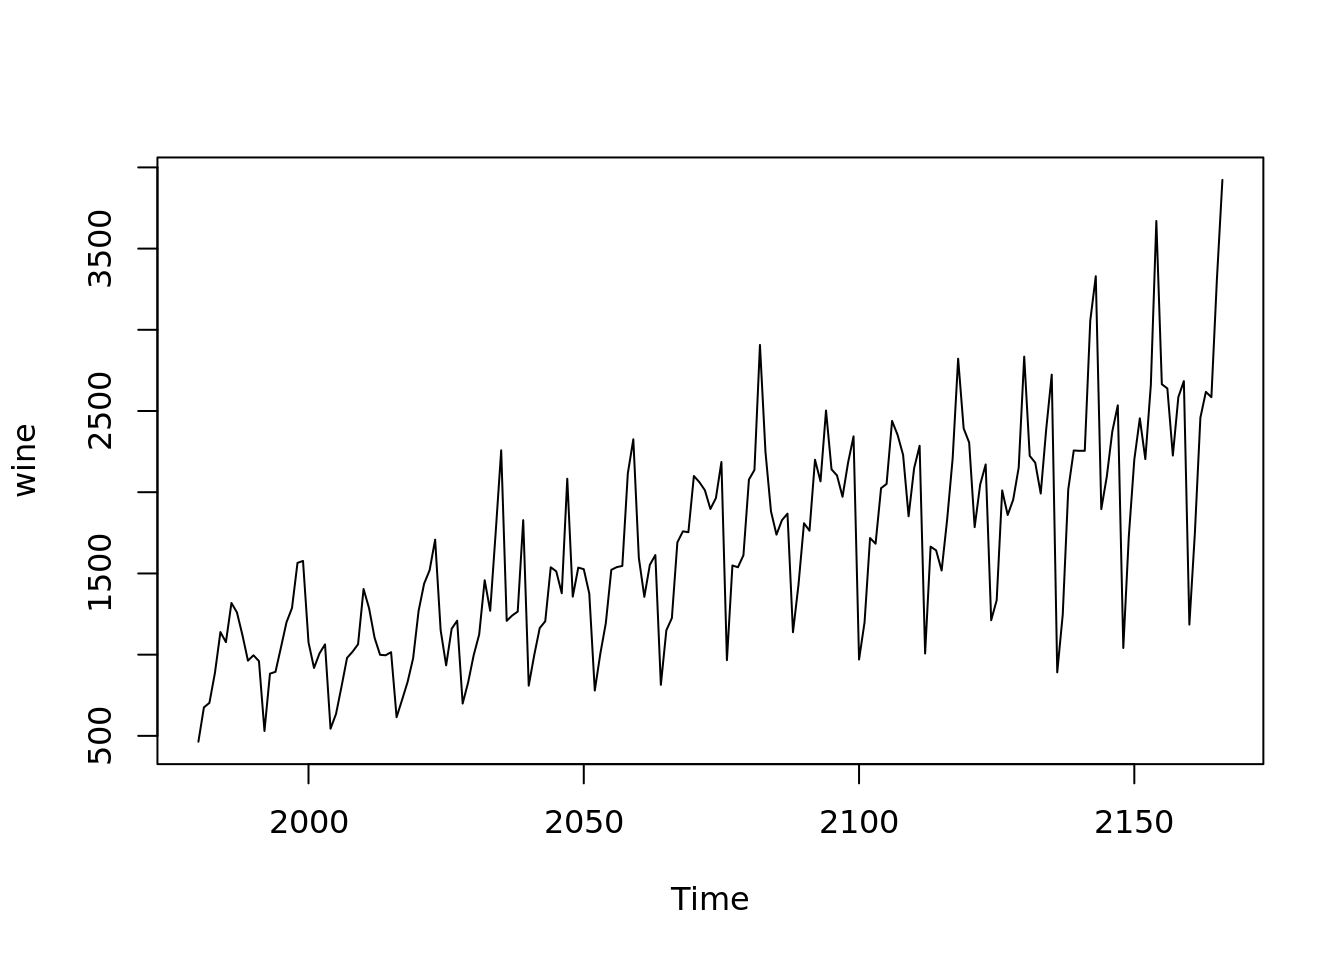
\includegraphics{Homework1_files/figure-latex/unnamed-chunk-3-1.pdf}

\begin{Shaded}
\begin{Highlighting}[]
\FunctionTok{acf}\NormalTok{(Z)}
\end{Highlighting}
\end{Shaded}

\includegraphics{Homework1_files/figure-latex/unnamed-chunk-3-2.pdf}

\begin{enumerate}
\def\labelenumi{(\alph{enumi})}
\setcounter{enumi}{1}
\tightlist
\item
\end{enumerate}

\begin{Shaded}
\begin{Highlighting}[]
\FunctionTok{set.seed}\NormalTok{(}\DecValTok{39}\NormalTok{)}
\FunctionTok{ts.plot}\NormalTok{(Y)}
\end{Highlighting}
\end{Shaded}

\includegraphics{Homework1_files/figure-latex/unnamed-chunk-4-1.pdf}

\begin{Shaded}
\begin{Highlighting}[]
\FunctionTok{acf}\NormalTok{(Y)}
\end{Highlighting}
\end{Shaded}

\includegraphics{Homework1_files/figure-latex/unnamed-chunk-4-2.pdf}

\begin{enumerate}
\def\labelenumi{(\alph{enumi})}
\setcounter{enumi}{2}
\item
  Just by looking at both time series plots, I could tell that they were
  both stationary because the majority of the values fall on a
  horizontal line. For the plot of Z, the horizontal line looks to be at
  y=0, while the plot of Y looks to have a horizontal line at y=1. Also,
  neither plot seems to have seasonality. For the plots of the acf of
  both Y and Z, it appears that Y has larger spikes then Z, which makes
  sense because Y = \(Z^2\). In addition, the acf of Z appears to come
  from a gaussian white noise distribution because its spikes are all
  within the blue dotted lines.
\item
  ~ \[
  \begin{aligned}
  & Z = N(0,1)\\
  & Y = Z_{t}^2\\
  E[Y] & = µ_{y}(t)\\
  E[Y] & = E[Z_{t}^2]\\
  & = Var[Z_{t}]+E[Z_{t}]^2\\
  & = 0 + 1\\
  &=1
  \end{aligned}
  \]\\
\end{enumerate}

\[
\begin{aligned}
For\ X &= N(0,\sigma^2),\ E[X^4]=3(\sigma^2)^2\\
Var[Y] & = \sigma^2_{y}(t)\\
Var[Y] & = Var[Z_{t}^2]\\
& = E[(Z_{t}^2)^2]-E[Z_{t}^2]^2\\
& = E[Z_{t}^4]-E[Z_{t}^2]^2\\
& = 3(1)^2 - 1^2\\
& = 2\\
\end{aligned}
\]/

\[
\begin{aligned}
& Assuming\ h=0\\
& If\ Cov(Z_{t},\ Z_{s})=0\ for\ t \ne s\ \rightarrow\ Cov(Z^2_{t},\ Z^2_{s})=0\\
&\rho_{Y}(t, t+h)=Cor(Y_{t}, Y_{t+h})\\ \\
&Cor(Y_{t}, Y_{t+h}) = \frac{Cov(Y_{t}, Y_{t+h})}{\sqrt{Var(Y_{t})*Var(Y_{t+h})}}\\ \\
& \ \ \ \ \ \ \ \ \ \ \ \ \ \ \ \ \ \ \ \ \ \ = \frac{Cov(Z^2_{t},\ Z^2_{t+h})}{\sqrt{Var(Y_{t})*Var(Y_{t+h})}}\\ \\
& \ \ \ \ \ \ \ \ \ \ \ \ \ \ \ \ \ \ \ \ \ \  = \frac{0}{\sqrt{2*2}}\\ \\
& \ \ \ \ \ \ \ \ \ \ \ \ \ \ \ \ \ \ \ \ \ \  = 0
\end{aligned}
\]\\

\setlength{\leftskip}{0cm}\\

\textbf{The following two problems are for students enrolled in PSTAT
274 ONLY}\\

\hypertarget{question-g1}{%
\paragraph{Question G1}\label{question-g1}}

Let \{Zt\} be \emph{Gaussian} white noise, i.e.~\{Z\textsubscript{t}\}
is a sequence of i.i.d. normal r.v.s each with mean zero and variance 1.

\setlength{\leftskip}{2cm}

Define:
\(X_t= \begin{cases}Z_t, & \text { if } t \text { is even } \\ \left(Z_{t-1}^2-1\right) / \sqrt{2}, & \text { if } t \text { is odd }\end{cases}\)

\setlength{\leftskip}{0cm}

Show that \{X\textsubscript{t}\} is WN(0, 1) (that is, variables
X\textsubscript{t} and X\textsubscript{t+k}, k ≥ 1, are uncorrelated
with mean zero and variance 1) but that X\textsubscript{t} and
X\textsubscript{t−1} are \textbf{not} i.i.d.\\

\[
\begin{align*}
Z_{t} \sim WN(0, 1)
\end{align*}
\]

\[
X_t= \begin{cases}Z_t, & \text { if } t \text { is even } \\ \left(Z_{t-1}^2-1\right) / \sqrt{2}, & \text { if } t \text { is odd }\end{cases}
\]

\[ 
\begin{align*}
\text{If t is even}:&\\
& E[X_{t}] = E[Z_{t}]\\
&\ \ \ \ \ \ \ \ \ \ = 0\\
\text{If t is odd}:&\\
& E[X_{t}] = E[(Z^2_{t-1}-1)/\sqrt{2}]\\
&\ \ \ \ \ \ \ \ \ \ = \sqrt{2}\ (E[Z^2_{t-1}]-1)\\
&\ \ \ \ \ \ \ \ \ \ = \sqrt{2}\ (Var[Z_{t-1}]+E[Z_{t-1}]^2-1)\\
&\ \ \ \ \ \ \ \ \ \ = \sqrt{2}\ (1+(0)^2-1)\\
&\ \ \ \ \ \ \ \ \ \ = 0
\end{align*}
\]

\[ 
\begin{align*}
\text{If t is even}:&\\
& Var[X_{t}] = Var[Z_{t}]\\
&\ \ \ \ \ \ \ \ \ \ \ \ \ \ = 1\\
\text{If t is odd}:&\\
& Var[X_{t}] = Var[(Z^2_{t-1}-1)/\sqrt{2}]\\
&\ \ \ \ \ \ \ \ \ \ \ \ \ \ = \frac{1}{2}\ (Var[Z^2_{t-1}])\\
&\ \ \ \ \ \ \ \ \ \ \ \ \ \ = \frac{1}{2}\ (E[Z_{t-1}^4]-E[Z^2_{t-1}]^2])\\
&\ \ \ \ \ \ \ \ \ \ \ \ \ \ = \frac{1}{2}\ (3(Var[Z_{t-1}])^2-(Var[Z_{t-1}]-E[Z_{t-1}])^2)\\
&\ \ \ \ \ \ \ \ \ \ \ \ \ \ = \frac{1}{2}\ (3(1)^2-(1-0^2)^2)\\
&\ \ \ \ \ \ \ \ \ \ \ \ \ \ = \frac{1}{2}\ (2)\\
&\ \ \ \ \ \ \ \ \ \ \ \ \ \ = \ 1\\
\end{align*}
\]

\[
\begin{align*}
&E[X_{t}] = \begin{cases}E[Z_t] = 0, & \text { if } t \text { is even } \\ \left(E[(Z_{t-1}^2-1\right) / \sqrt{2}] = 0, & \text { if } t \text { is odd }\end{cases}\\
& \ \ \ \ \ \ \ \ \ \ = 0\\ \\
&Var[X_{t}] = \begin{cases}Var[Z_t] = 1, & \text { if } t \text { is even } \\ \left(Var[(Z_{t-1}^2-1\right) / \sqrt{2}] = 1, & \text { if } t \text { is odd }\end{cases}\\
& \ \ \ \ \ \ \ \ \ \ \ \ \ \ = 0\\ \\
& \rightarrow\ X_{t} \sim WN(0,1)
\end{align*}
\]\\

\[
\begin{align*}
& \text{Let t be even and h be odd} \\
&Cor(X_{t}, X_{t+h}) = \frac{Cov(X_{t}, X_{t+h})}{\sqrt{Var(X_{t})*Var(X_{t+h})}}\\ \\
&\text{Since}\ X_{t}\ \ \&\ \ X_{t+h}\ \ \text{are both from the distribution WN(0,1)} \\
& \ \ \ \ \ \ \ \ \ \ \ \ \ \ \ \ \ \ \ \ \ \ \ \ \ \ \ \ \ \ \ \ \ \ \ \ \ \ \ \ \ \& \\
& \ \ \ \ \ \ \ \ \ \ Cov[(WN_{t}(0,1),\ WN_{s}(0,1)]=0\ for\ t \ne s\ \\ \\
& \ \ \ \ \ \ \ \ \ \ \text{Then}\ \ Cov(X_{t}, X_{t+h})=0 \\
& \ \ \ \ \ \ \ \ \ \ \ \ \ \ \ \rightarrow Cor(X_{t}, X_{t+h}) = 0\\ \\
&\text{Thus,}\ X_{t}\ \text{and}\ X_{t+h}\ \text{are uncorrelated}.\\
&\text{But because}\ X_{t+h} = (Z^2_{t-1+h}-1)/\sqrt{2}\ \text{and}\ Z^2_{t-1+h}\ \text{is dependent on}\ Z_{t+h-1,}\\
&\text{then}\ X_{t+h}\ \text{is also dependent on}\ X_{t+h-1}. \\
&\text{Therefore,}\ X_{t}\ \text{and}\ X_{t+h}\ \text{are not i.i.d. variables.}
\end{align*}
\] ~\\

\hypertarget{question-g2}{%
\paragraph{Question G2}\label{question-g2}}

If \{X\textsubscript{t}\} and \{Y\textsubscript{t}\} are uncorrelated
stationary sequences, i.e., if X\textsubscript{r} and Y\textsubscript{s}
are uncorrelated for every r and s, show that \{X\textsubscript{t} +
Y\textsubscript{t}\} is stationary with autocovariance function equal to
the sum of the autocovariance functions of \{X\textsubscript{t}\} and
\{Y\textsubscript{t}\}.

\[
\begin{aligned}
& \text{Given that both time series are uncorrelated, their covariance is 0}. \\
& \rightarrow\ Var(X_{t}\ +\ Y_{t}) = Var(X_{t}) + Var(Y_{t}) \\
& \rightarrow\ E(X_{t}\ +\ Y_{t}) = E(X_{t}) + E(Y_{t})\\
& \ \ \ \ \ \ \ \ \ \ \ \ = µ_{X}+_{Y}\\
&\gamma_{X+Y}(h) = Cov(X_{t}+Y_{t},\ X_{t+h}+Y_{t+h})\\
& \ \ \ \ \ \ \ \ \ \ \ \ \ \ = Cov(X_{t},\ X_{t+h})\ +\ Cov(X_{t},\ Y_{t+h})\ +\ Cov(Y_{t},\ X_{t+h})\ +\ Cov(Y_{t},\ Y_{t+h})\\
&\ \ \ \ \ \ \ \ \ \ \ \ \ \ = Cov(X_{t},\ X_{t+h})\ +\ Cov(Y_{t},\ Y_{t+h}) \\
&\ \ \ \ \ \ \ \ \ \ \ \ \ \  = \gamma_{X}(h) + \gamma_{Y}(h)\\ \\
&\text{Given that we already know that both time series are stationary and the}\\
&\text{autocovariance of their sum is the sum of their autocovariances, the sum of their}\\
&\text{constant stationary coefficients will also be constant and therefore stationary.}
\end{aligned}
\]

\end{document}
